\documentclass{beamer}

\setbeamertemplate{caption}[numbered]

\mode<presentation> {
\usetheme{Madrid}
}

\usepackage{graphicx} % Allows including images
\usepackage{booktabs} % Allows the use of \toprule, \midrule and \bottomrule in tables}
\usepackage{amsmath}
\usepackage{xcolor}
\usepackage{physics}
%----------------------------------------------------------------------------------------
%	TITLE PAGE
%----------------------------------------------------------------------------------------

\title[Wobbling Motion in odd-A nuclei]{A Novel Approach for the Semi-Classical Description of the Wobbling Properties in Odd-A Nuclei} % The short title appears at the bottom of every slide, the full title is only on the title page

\author{Robert Poenaru} % Your name
\institute[DFT] % Your institution as it will appear on the bottom of every slide, may be shorthand to save space
{
Department of Theoretical Physics, IFIN-HH \\
\vspace{0.1cm}
Faculty of Physics, University of Bucharest \\% Your institution for the title page
\medskip
\textit{robert.poenaru@drd.unibuc.ro} % Your email address
}
\date{\today} % Date, can be changed to a custom date

\begin{document}

\begin{frame}
\titlepage % Print the title page as the first slide
\end{frame}

\begin{frame}
\frametitle{Outline} % Table of contents slide, comment this block out to remove it
\tableofcontents % Throughout your presentation, if you choose to use \section{} and \subsection{} commands, these will automatically be printed on this slide as an overview of your presentation
\end{frame}


\section{Wobbling Motion} 

\begin{frame}{Shape parametrization}
Nuclear shapes can be described via the \textbf{quadrupole parameter} $\beta$ and the \textbf{triaxiality parameter} $\gamma$.
\begin{figure}
    \centering
    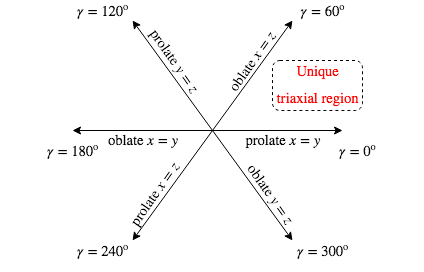
\includegraphics[scale=0.5]{figs/beta_gamma_plane.png}
    \caption{The $(\beta,\gamma$) plane divided into six equivalent parts.}
    \label{betagamma}
\end{figure}
\end{frame}

\begin{frame}{Nuclear shapes}
Nuclear shapes: most of the nuclei are spherical or axially symmetric in the ground state.
  \begin{figure}
    \centering
    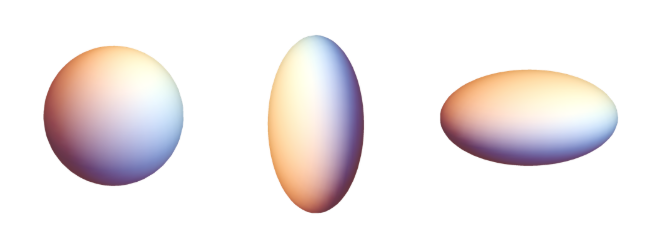
\includegraphics[scale=0.4]{figs/nuclear_shapes.png}
    \caption{\textbf{Spherical:} $\beta_2=0$ ; \textbf{Prolate:} $\beta_2>0$ ; \textbf{Oblate:} $\beta_2<0$}
  \end{figure}
  \begin{exampleblock}{Triaxial shapes}
       There are also deviations from \emph{axial symmetric shapes} $\to$ \textbf{triaxial shapes} (e.g. no symmetry axis). The three PA's have different lengths.
  \end{exampleblock}
\end{frame}

% \begin{frame}{Wobbling motion}
% \begin{columns}
%     \begin{column}{0.5\textwidth}
%     \begin{block}{Wobbling motion (WM)}
%   \begin{itemize}
%     \item Uniquely associated to triaxial structures. 
%     \item It was theoretically predicted by Bohr and Mottelson more than 50 years ago (for the even-$A$ case).
%     \item Experimentally confirmed for $^{163}$Lu in 2001.
%   \end{itemize}
%   \end{block}
%   \begin{exampleblock}{Experimental evidence}
%   In present, few wobblers are experimentally confirmed in the mass regions: $A\approx130,160,180$.
%   \end{exampleblock}
%   \end{column}
%   \begin{column}{0.5\textwidth}
%         \begin{figure}
%           \centering
%           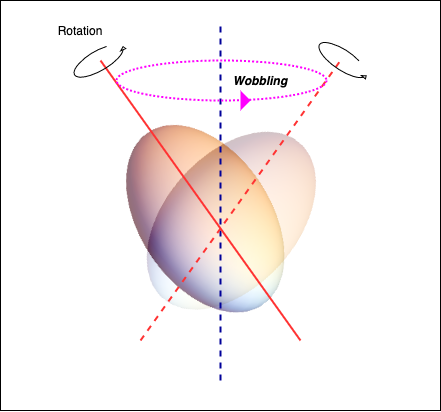
\includegraphics[scale=0.35]{figs/wobbling_drawing.png}
%           \caption{Schematic representation for the nuclear wobbling motion.}
%           \label{wobbling_picture}
%       \end{figure}
%   \end{column}
%   \end{columns}
% \end{frame}

\begin{frame}{Wobbling motion}

\begin{block}{Wobbling motion (WM)}
  \begin{itemize}
    \item Uniquely associated to triaxial structures. 
    \item It was theoretically predicted by Bohr and Mottelson more than 50 years ago (for the even-$A$ case).
    \item This motion has an oscillating behavior.
    \item Spectrum: $E=E_\text{rot}+E_\text{wob}\left(n_w+\frac{1}{2}\right)$.
  \end{itemize}
  \end{block}
  \begin{exampleblock}{Experimental evidence}
  \begin{itemize}
  \item Experimentally confirmed for $^{163}$Lu in 2001.
  \item In present, few wobblers are experimentally confirmed in the mass regions: $A\approx130,160,180$.
  \end{itemize}
  \end{exampleblock}
\end{frame}

\begin{frame}{Wobbling motion}
  \begin{columns}
    \begin{column}{0.47\textwidth}
    \begin{block}{Triaxial nuclei}
        A triaxial nucleus can rotate about any of the three axes.
        
        \vspace{0.3cm}
        
        The rotational angular momentum is NOT aligned along any of the body-fixed axes: it \textbf{precesses} and \textbf{wobbles} around the axes with the largest MOI. 
    \end{block}
    \end{column}
    \begin{column}{0.53\textwidth}  %%<--- here
%   \begin{figure}
%      \centering
%      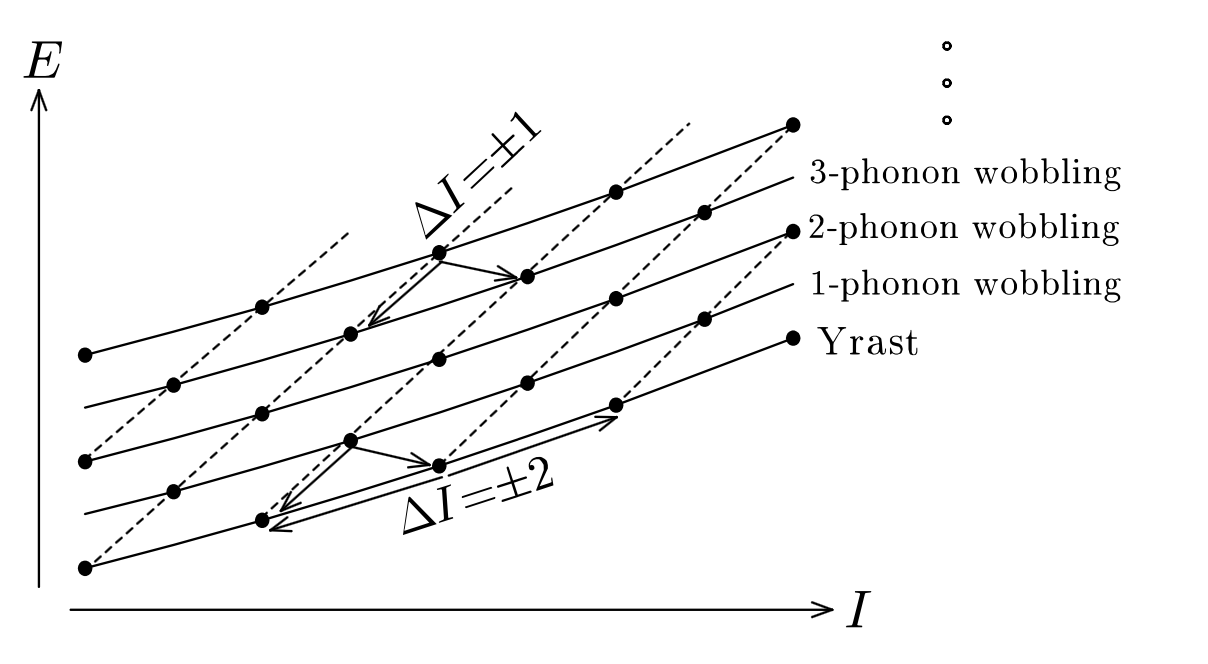
\includegraphics[scale=0.15]{figs/wobblingBands.png}
%      \caption{Rotational-band structures of the wobbling motion.}
%   \end{figure}
         \begin{figure}
          \centering
          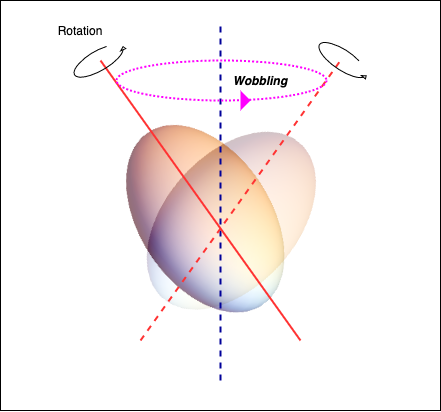
\includegraphics[scale=0.35]{figs/wobbling_drawing.png}
          \caption{Schematic representation for the nuclear wobbling motion.}
          \label{wobbling_picture}
      \end{figure}
  
    \end{column}
    \end{columns}
\end{frame}

\begin{frame}
\frametitle{Wobbling Bands}

\begin{columns} 
\column{.5\textwidth} 
\begin{block}{Wobbling bands}
  Sequences of $\Delta I=2\hbar$ rotational bands that are built on different \textit{wobbling phonon excitations}.
  
\end{block}

\begin{exampleblock}{Experimental evidence}
    $^{163}$Lu has \textbf{four} such wobbling bands, with $n_w=0,1,2,3$ wobbling phonon numbers, respectively.
\end{exampleblock}

\column{.5\textwidth}
\begin{figure}
     \centering
     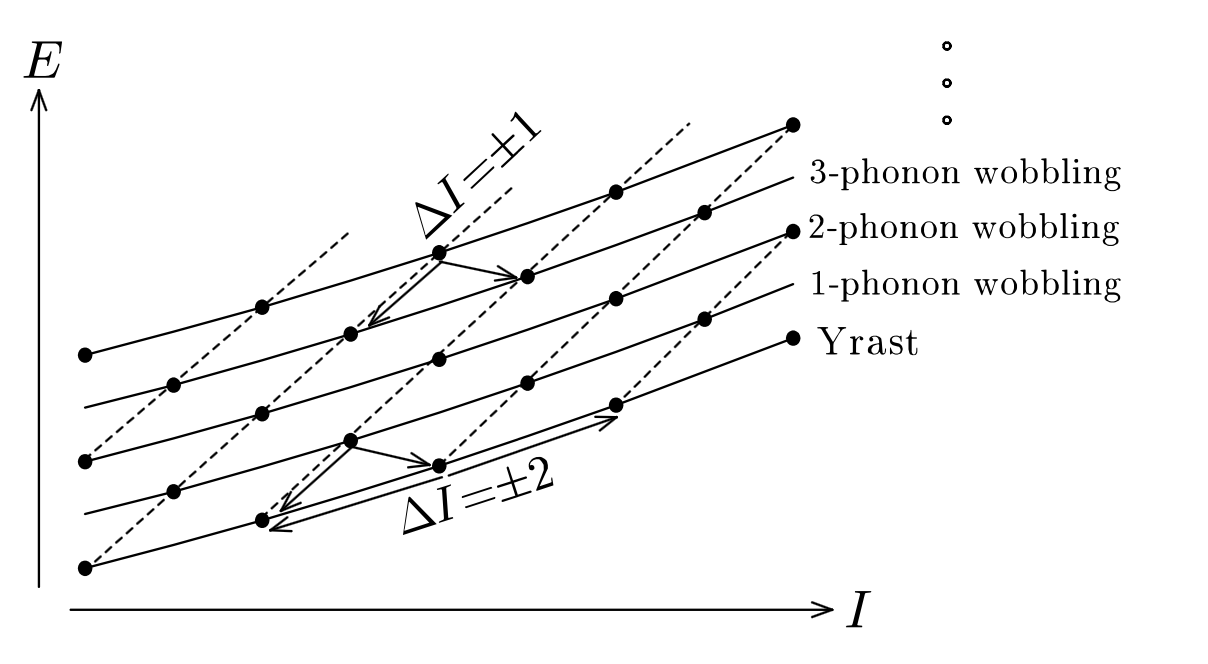
\includegraphics[scale=0.14]{figs/wobblingBands.png}
     \caption{Rotational-band structures of the wobbling motion.}
   \end{figure}
\end{columns}
\end{frame}

\begin{frame}{Particle-rotor coupling}
  \begin{block}{Wobbling motion in odd-A nuclei}  
    \begin{itemize}
      \item Coupling of a nucleon from a high j-shell with the triaxial rotor core is crucial for the wobbling phenomenon.
      \item The odd particle’s angular momentum couples to the rotor, driving the nucleus to large deformations and it also stabilizes the shape.
    \end{itemize}
  \end{block}
  \begin{exampleblock}{Odd particle}
  \begin{itemize}
      \item For nuclei with $A\approx160$, the odd $\pi i_{13/2}$ is the \emph{intruder} which drive the isotope to very high deformations (up to $n_w=3$ wobbling phonon number).
      \item The fourth wobbling band in $^{163}$Lu was considered to emerge from the coupling of a core with the $\pi h_{9/2}$ (Jensen et al), $\pi h_{11/2}$ (Frauendorf et al), or even $\pi h_{11/2}$ (Tanabe et al 2006).
    %   \item For nuclei with $A\approx180$, the odd $\pi h_{9/2}$ and $\pi i_{13/2}$ are the \emph{intruders} which drive the system to very high deformations.
  \end{itemize}
  \end{exampleblock}
\end{frame}

\begin{frame}{Theoretical framework}
  The odd-mass system consists of an {\color{red}even-even core} (described by a triaxial rotor Hamiltonian {\color{red}$H_\text{rot}$}) and a single {\color{blue}$j$-shell nucleon} described by its single-particle Hamiltonian {\color{blue}$H_\text{sp}$}.
  \par \textbf{Total system:}
  \begin{align}
    &H={\color{red}H_\text{rot}}+{\color{blue}H_\text{sp}}=\\
&{\color{red}\sum_{k=1,2,3}A_k(I_k-j_k)^2}+{\color{blue}\epsilon_j+\frac{V}{j(j+1)}\left[\cos\gamma(3j_3^2-\mathbf{j}^2)-\sqrt{3}\sin\gamma(j_1^2-j_2^2)\right]}
  \end{align}
  \par {\footnotesize \textbf{Solving the Hamiltonian in semi-classical approach for $^{163}Lu$}: \textit{R. Poenaru and A. A. Raduta, International Journal of Modern Physics E, 2150033, \textbf{2021}}.}
  \par {\footnotesize \textbf{For $^{135}Pr$}: \textit{A. A. Raduta and R. Poenaru, Journal of Physics G, 015106, \textbf{2020}}.}
\end{frame}

\begin{frame}{Energy function - Semiclassical approach}
      The eigenvalues for $\hat{H}=H_{rot}+H_{sp}$ are obtained by solving the \emph{variational principle}:
  \begin{align}
    \delta \int_0^t\bra{\Psi_{IjM}}\hat{H}-i\frac{\partial}{\partial t'}\ket{\Psi_{IjM}}dt'=0. \label{varp}
  \end{align}
  The trial function $\ket{\Psi_{IjM}}$ is a direct product $\ket{\psi}_\text{core}\otimes\ket{\phi}_\text{s.p.}$.
    From Eq. \ref{varp}, one obtains the \emph{classical equations of motion} in the canonical form:
  \begin{align}
    \frac{\partial \mathcal{H}}{\partial r}=\dot{\varphi}\ ;\ \frac{\partial\mathcal{H}}{\partial\varphi}=-\dot{r}\\
    \frac{\partial \mathcal{H}}{\partial t}=\dot{\psi}\ ;\ \frac{\partial\mathcal{H}}{\partial \psi}=-\dot{t}
  \end{align}
\end{frame}

\begin{frame}{Semiclassical wobbling energies}
\begin{block}{Harmonic Frequencies}
\begin{itemize}
    \item They represent the harmonic-like behavior of the wobbling motion in odd-A nuclei.
  \item In our model, the pair of frequencies $({\color{blue}\Omega_1^I},{\color{red}\Omega_{2}^I})$ is associated with the rotational motion of the {\color{blue}core} and the {\color{red}odd particle}, respectively.
\end{itemize}
\end{block}
\begin{alertblock}{Energy spectrum}
\begin{align}
    E_I&={\color{cyan}\epsilon_{j}}+{\color{magenta}\mathcal{H}_\text{min}(I)}+\left[{\color{blue}\Omega_1^I\left(n_{w_1}+\frac{1}{2}\right)}+{\color{red}\Omega_2^I\left(n_{w_2}+\frac{1}{2}\right)}\right] \label{wobbling_formula}
  \end{align} 
  Terms: {\color{cyan}{single particle energy}}, {\color{magenta}energy in the minimum point} and [harmonic-like motion].
\end{alertblock}
\end{frame}

\section{Unique features}

\begin{frame}{Characteristics of the model}
    \begin{block}{Existing interpretation of WM in $^{163}$Lu}
    \begin{itemize}
        \item $n_{w_1}=0$, $n_{w_2}=1$, $n_{w_3}=2$, $n_{w_4}=3$
        \item TSD1-3: rotor couples with $j=13/2$ proton. TSD4: rotor couples with $j=9/2$ proton.
        \item The moments of inertia for band TSD4 differ than TSD1-3
    \end{itemize}
    \end{block}
    \begin{alertblock}{New (current) approach}
    \begin{itemize}
        \item TSD1 and TSD2 are \emph{signature partner bands} $\to$ $n_{w_1}=0$, $n_{w_2}=0$
        \item TSD3 is one-phonon wobbling band built on top of TSD2. $n_{w_3}=1$
        \item Same $j=13/2$ proton occurs in the particle-rotor coupling for all four bands.
        \item TSD2 and TSD4 are \emph{parity partner bands} ($n_{w_2}=0$, $n_{w_4}=0$). Same structure but opposite parity $\to$ The triaxial rotor admits \textbf{wave-functions} of both parities.
    \end{itemize}
    \end{alertblock}
\end{frame}

\section{Numerical results}

\begin{frame}{Excitation energies I}
\small{\emph{R. Poenaru, A. A. Raduta, Romanian Journal of Physics 66, 308, \textbf{2021}.}}
\begin{columns} 
\column{.5\textwidth} 
\begin{figure}
    \centering
    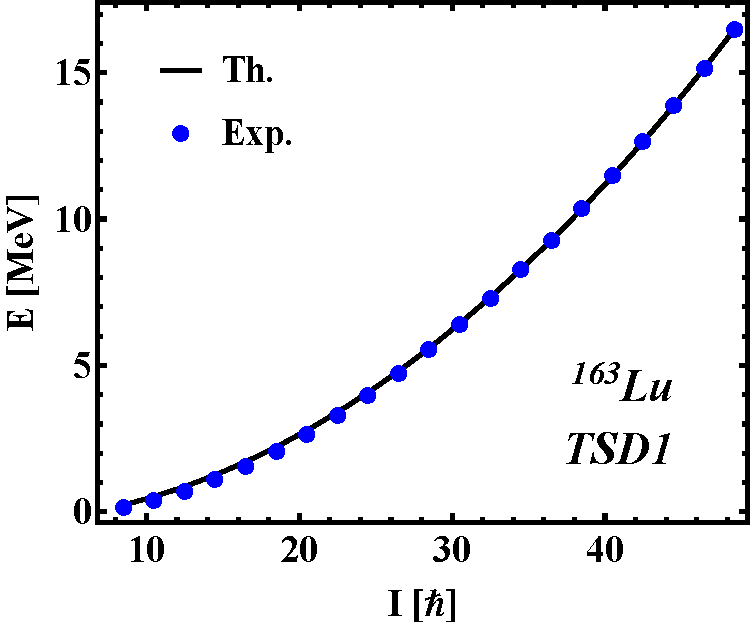
\includegraphics[scale=0.4]{figs/DoubleShift_TSD1.pdf}
    \caption{The excitation energies for the band TSD1.}
\end{figure}
\column{.5\textwidth}
\begin{figure}
    \centering
    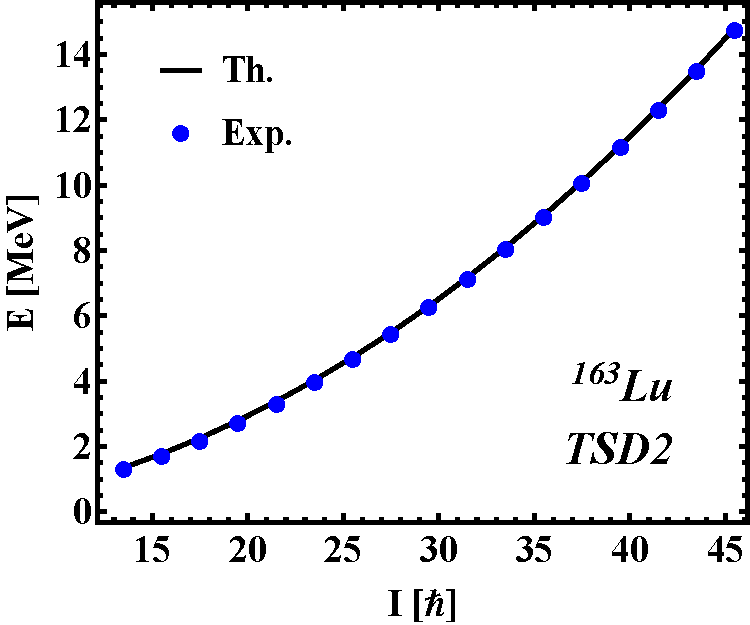
\includegraphics[scale=0.4]{figs/DoubleShift_TSD2.pdf}
    \caption{The excitation energies for the band TSD2.}
\end{figure}
\end{columns}
Parameters: $\mathcal{I}_1=72$, $\mathcal{I}_2=15$, $\mathcal{I}_3=7$ $\hbar^2$/MeV. $\gamma=22^\circ$. $V=2.1$ MeV.
\end{frame}

\begin{frame}{Excitation energies II}
\small{\emph{R. Poenaru, A. A. Raduta, Romanian Journal of Physics 66, 308, \textbf{2021}.}}
    \begin{columns} 
\column{.5\textwidth} 
\begin{figure}
    \centering
    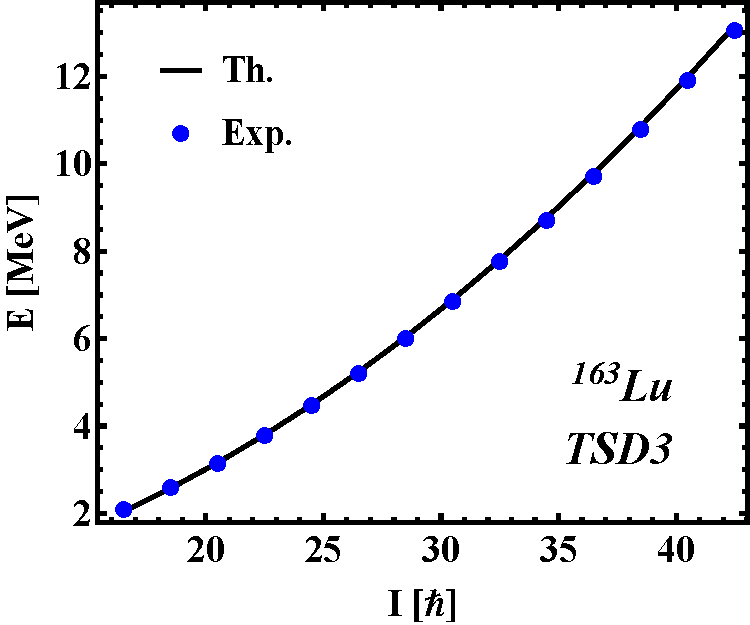
\includegraphics[scale=0.4]{figs/DoubleShift_TSD3.pdf}
    \caption{The excitation energies for the band TSD3.}
\end{figure}
\column{.5\textwidth}
\begin{figure}
    \centering
    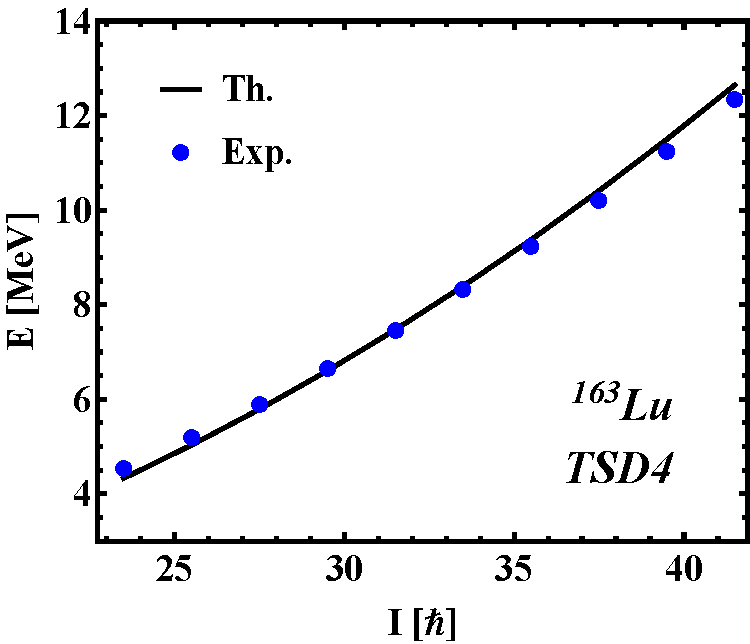
\includegraphics[scale=0.4]{figs/DoubleShift_TSD4.pdf}
    \caption{The excitation energies for the band TSD4.}
\end{figure}
\end{columns}
\end{frame}

\begin{frame}{Wobbling energies + frequencies}
\begin{columns} 
\column{.5\textwidth}
\begin{figure}
    \centering
    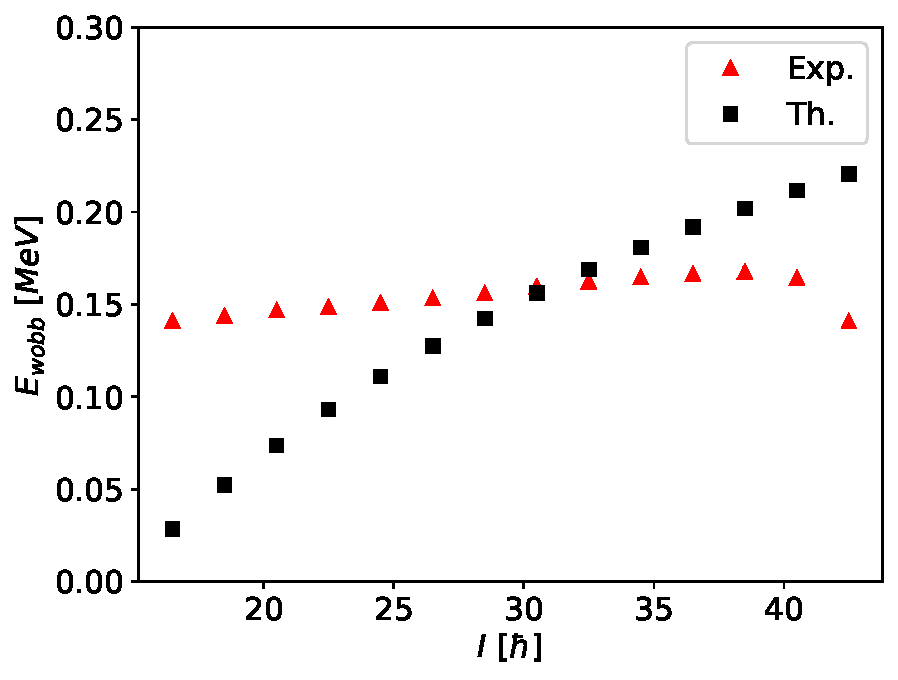
\includegraphics[scale=0.38]{figs/wobbling_energy_ThExp.pdf}
    \caption{The wobbling energies for $^{163}$Lu given as formula below. $E_1$ belong to $TSD_3$, while $E_0$ correspond to $TSD_2$.}
    \label{wobbling-energies_th_exp}
\end{figure}
\column{.5\textwidth}
\begin{figure}
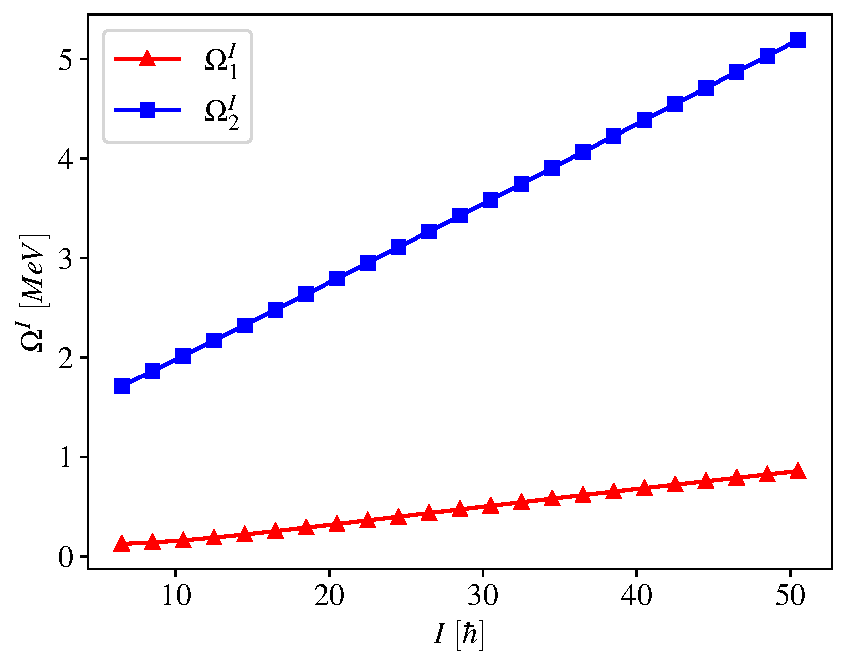
\includegraphics[scale=0.4]{figs/wobbling-frequencies.pdf}
\caption{The wobbling frequencies as function of total angular momentum.}
\end{figure}
\end{columns}
$$E_\text{wob}=E_1(I)-\frac{1}{2}(E_0(I+1)+E_0(I-1))$$
\end{frame}

\begin{frame}{Classical energy function - contour plots I}
Spin: \textbf{Quantal $\to$ classical}. $I=I_1,I_2,I_3\ \to\ I=x_1,x_2,x_3$. \\
Spherical coordinates $\to$ $x_k=f(I_0,\theta,\varphi)$.\\
Express the $\mathcal{H}$ (average of the Hamiltonian on the trial function) in terms of $(\theta,\varphi)$.
    \begin{columns} 
\column{.5\textwidth}
\begin{figure}
    \centering
    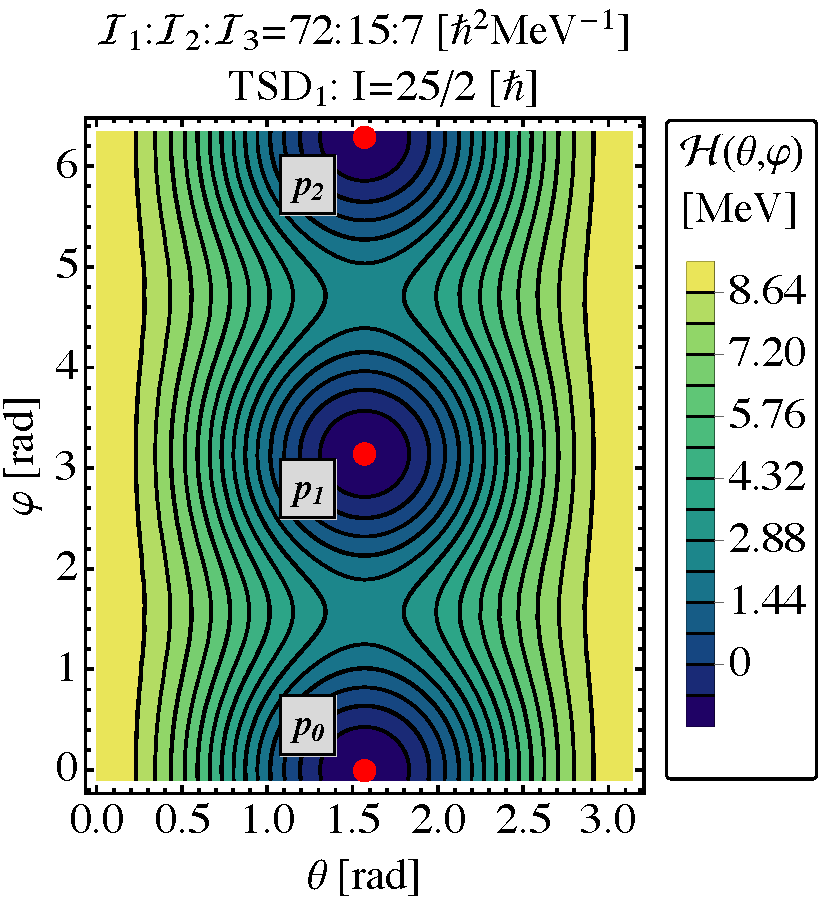
\includegraphics[scale=0.3]{figs/contour1_optimal.pdf}
    \caption{TSD1}
\end{figure}
\column{.5\textwidth}
\begin{figure}
    \centering
    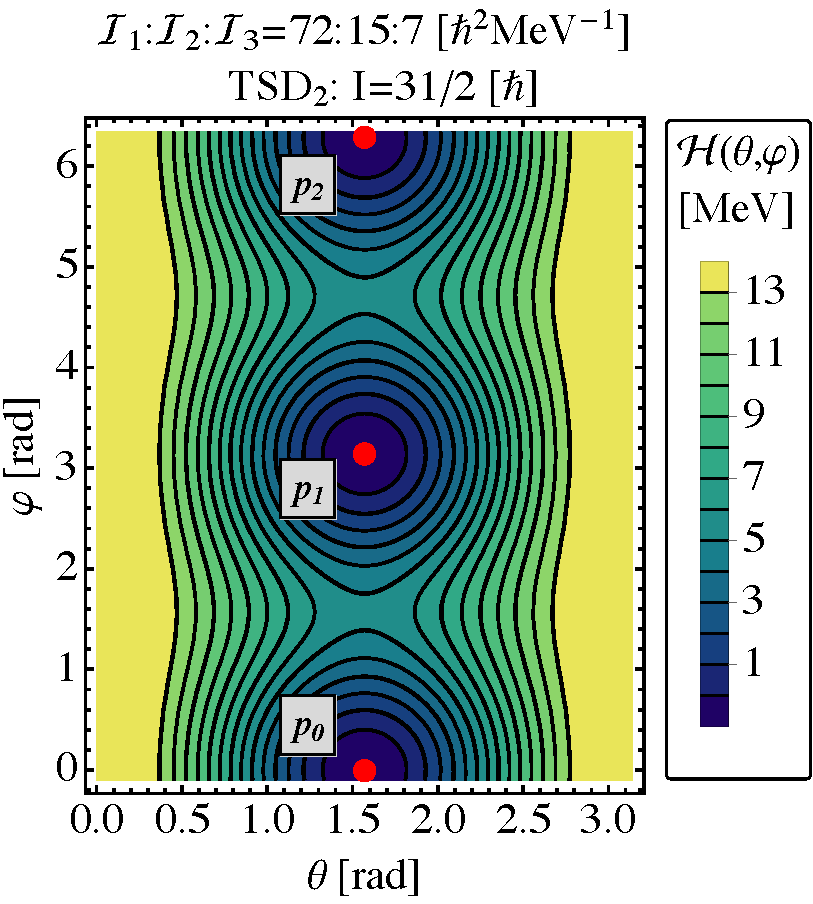
\includegraphics[scale=0.3]{figs/contour2_optimal.pdf}
    \caption{TSD2}
\end{figure}
\end{columns}
\end{frame}

\begin{frame}{Classical energy function - contour plots II}
    \begin{columns} 
\column{.5\textwidth}
\begin{figure}
    \centering
    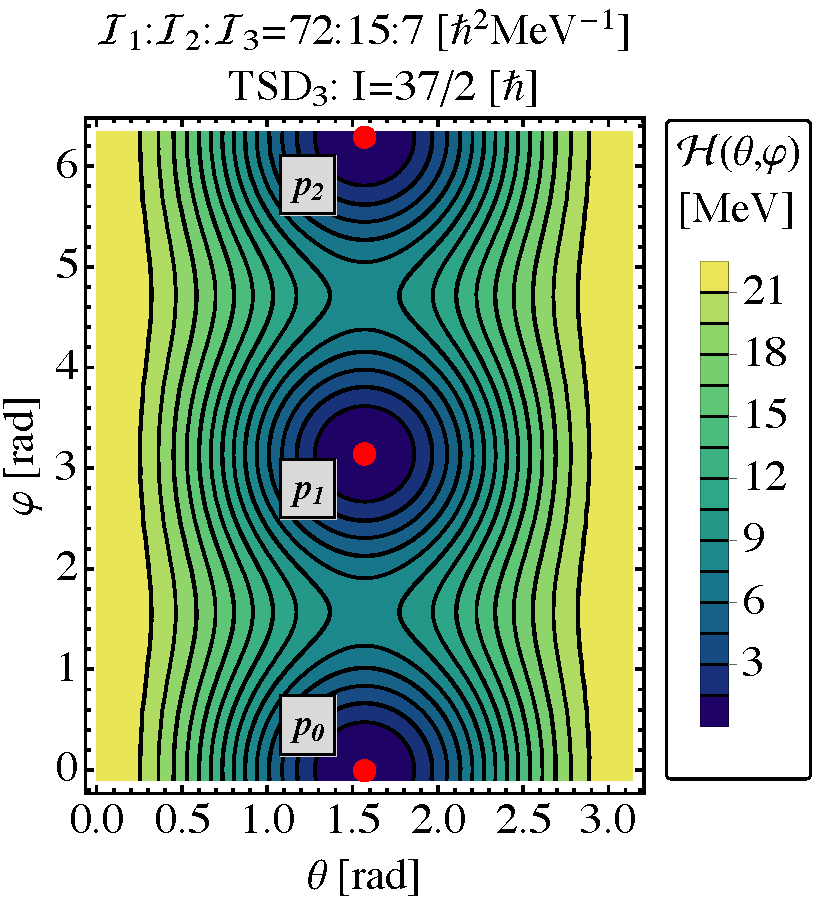
\includegraphics[scale=0.3]{figs/contour3_optimal.pdf}
    \caption{TSD3}
\end{figure}
\column{.5\textwidth}
\begin{figure}
    \centering
    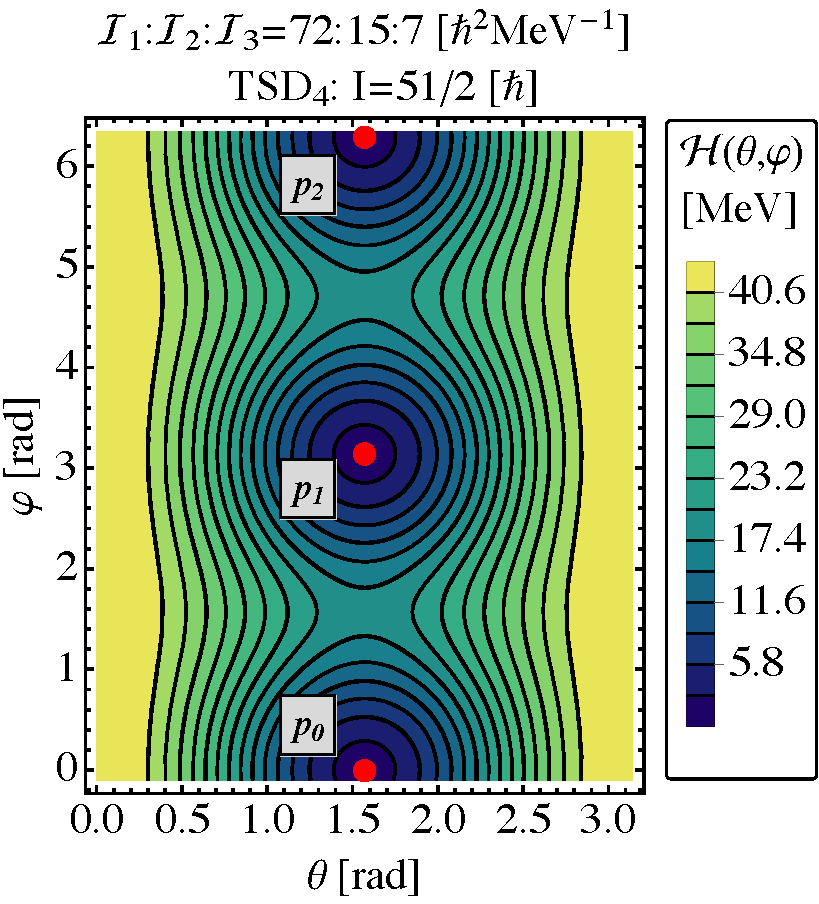
\includegraphics[scale=0.3]{figs/contour4_optimal.pdf}
    \caption{TSD4}
\end{figure}
\end{columns}
As the energy increases, the trajectories go around all minima.The lack of localization indicates unstable wobbling motion. 

\footnotesize{\textit{R. Poenaru, A. A. Raduta, Romanian Journal of Physics 66, 309 \textbf{2021}} - in press}
\end{frame}

\begin{frame}{Classical trajectories I}
3D representation of the angular momentum operator $\to$ Angular momentum sphere.\\
3D representation of $\mathcal{H}$ as a function of $x_1, x_2, x_3$. (the energy within a.m. space)
\begin{figure}
    \centering
    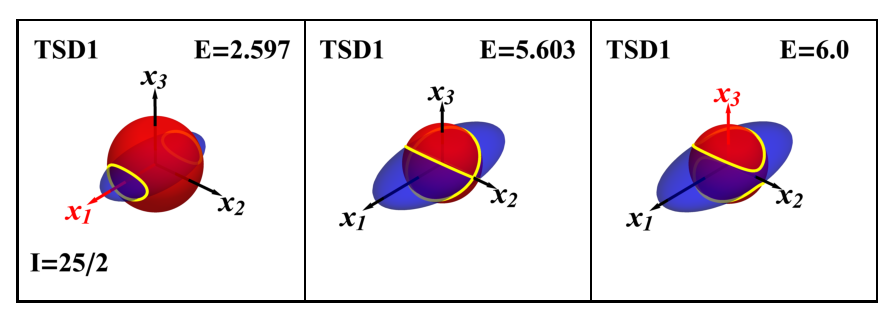
\includegraphics[scale=0.45]{figs/tsd1_spin1.eps}
    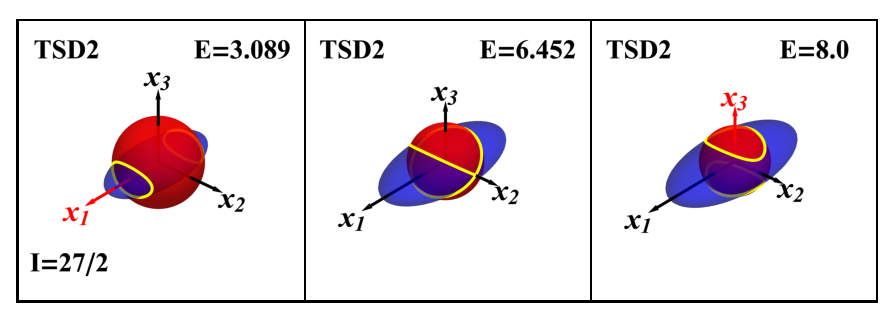
\includegraphics[scale=0.45]{figs/tsd2_spin1.eps}
    \caption{Intersection lines marked by yellow color represent the trajectories.}
\end{figure}
\end{frame}


\begin{frame}{Classical trajectories II}
\begin{figure}
    \centering
    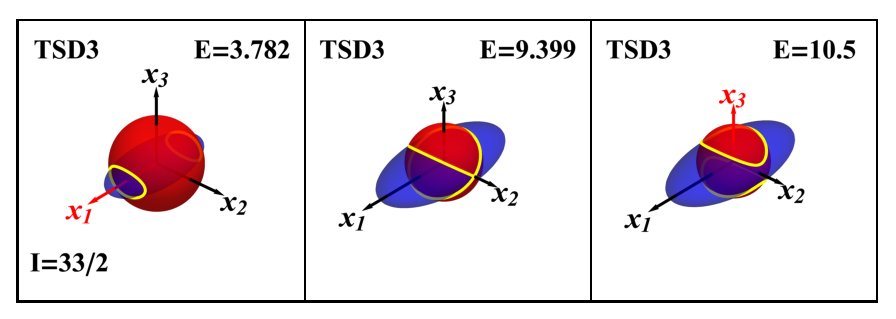
\includegraphics[scale=0.45]{figs/tsd3_spin1.eps}
    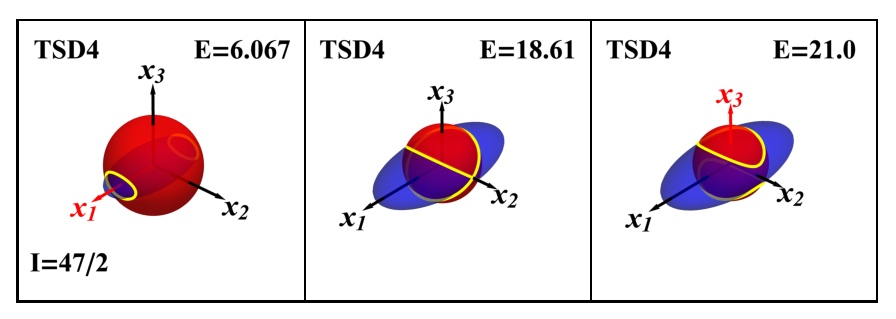
\includegraphics[scale=0.45]{figs/tsd4_spin1.eps}
    \caption{Intersection lines marked by yellow color represent the trajectories.}
\end{figure}
\footnotesize{\textit{R. Poenaru, A. A. Raduta, Romanian Journal of Physics 66, 309 \textbf{2021}} - in press}
\end{frame}

% \begin{frame}
% \frametitle{References}
% \footnotesize{
% \begin{thebibliography}{99} % Beamer does not support BibTeX so references must be inserted manually as below
% \bibitem[Smith, 2012]{p1} John Smith (2012)
% \newblock Title of the publication
% \newblock \emph{Journal Name} 12(3), 45 -- 678.
% \end{thebibliography}
% }
% \end{frame}

\begin{frame}
\Huge{\centerline{Thank you for your attention!}}
\end{frame}

\end{document} 